At low redshifts, peculiar velocities of galaxies can be directly measured 
and be used to learn about gravity on large scales. 
As presented in chapters~\ref{chap:intro} and \ref{chap:galaxies}, velocities 
are generally not observable other than by their indirect impact on the 
galaxy clustering through redshift-space distortions (RSD).
At $z<0.2$, the volume that can be probed by galaxy surveys is insufficient to obtain 
precise measurements of the growth-rate of structures $f$ solely with RSD. 
The additional information from peculiar velocities
significantly improves these constraints, to the point where one 
can perform consistency tests of the standard cosmological model or of our current 
model for gravity: general relativity. 

In this chapter I will expose the recent work we developed within the 
cosmology group at the Centre de Physique des Particules de Marseille 
in trying to combine galaxy surveys and peculiar velocities, 
particularly those obtained from type-Ia supernovae. Most of the work 
was carried out by the PhD student Bastien Carreres whom I co-supervise. 




\section{Measuring peculiar velocities}
\label{velocities:measuring}

As discussed in section~\ref{intro:probes:rsd}, 
redshifts of galaxies can be seen as a mixture of two distinct types of redshift. 
The first one is due to the expansion of the Universe and we refer to it as 
\emph{cosmological redshift} $z_\text{cos}$. The second one is due to Doppler effect and the peculiar 
velocities of galaxies with respect to a comoving frame, we refer to it as \emph{peculiar redshift} $z_\text{pec}$.
The total observed redshift $z_\text{obs}$ can be written as: 
\begin{equation}
    1+ z_\text{obs} = (1+z_\text{cos})(1+z_\text{pec})
\end{equation}

Measuring peculiar velocities or redshifts $z_\text{pec}$ means 
breaking the degeneracy between $z_\text{cos}$ and $z_\text{obs}$. 
The observed redshift of a given galaxy can be precisely measured via spectroscopy 
but its cosmological redshift requires a measurement of its distance or age, 
of which we can derive $z_\text{cos}$ through a cosmological model.
Therefore, peculiar velocity surveys can be seen simply as distance surveys.

Measuring distance of individual objects on cosmological scales is quite challenging
since it commonly involves standard or standardisable candles. 
For cosmological distances, three types of standardisable candles have been used by
peculiar velocity surveys: spiral galaxies, elliptical galaxies and type-Ia supernovae. 
Many decades of studies of galaxies have pointed to interesting correlations 
between their luminosity or absolute magnitudes, which are not directly observable,
to properties or physical quantities that can be directly observed and do not depend on 
the galaxy distance. 
Two famous correlations are the Tully-Fisher (TF) relation for spiral galaxies 
and the Fundamental Plane (FP) for ellipticals, which we will describe shortly after. 
Needless to say, type-Ia supernovae (SNIa) have been proven to be excellent standardisable candles
when accounting for correlations between their luminosity and the duration and colour of their light-curves. 
As discussed in section~\ref{intro:probes:snia}, SNIa are by themselves a key cosmological probe of 
the Universe's expansion. 

The precision of distance measurements is highly dependent on the modelling of correlations 
between luminosity, from which we derive luminosity distances, and their observed properties. 
Even after standardisation, each method remains with some intrinsic scatter in distances. 
For instance, TF and FP distances have generally a scatter of about 20\% while SNIa 
can reduce it to about 8\%. For cosmological applications, one SNIa distance is worth 4 to 5 
TF or FP distances to obtain the same precision. 
 

    \subsection{The Tully-Fisher relation of spiral galaxies} 
    \label{velocities:measuring:tf}
    
    The Tully-Fisher relation is an empirical link between the mass of spiral galaxies 
    and their rotational velocity at the regime where it does not vary much with distance to 
    the center. \cite{tullyNewMethodDetermining1977} where the first to find a correlation 
    between a distance-independent observable, the asymptotic rotational velocity, and 
    mass or luminosity, and to use it as a method to infer galaxy distances. 
    The physical origin of the relation is the virial theorem of a collapsed object. 

    Later works found that the infrared luminosity correlates better with rotational 
    velocity, i.e., it reduces the remaining scatter. This is because infrared wavelengths 
    are less sensitive to dust extinction than optical wavelengths.  
    \cite{mcgaughBaryonicTullyFisherRelation2000} have later shown that the standard 
    Tully-Fisher relation breaks down for galaxies with small rotation velocities. 
    However, those galaxies contain relatively more gas than stars. If the total baryonic mass 
    is used instead of only stellar mass, the relation holds even for these smaller galaxies. 
    This is known today as the baryonic Tully-Fisher (BTF) relation. 

    One of the largest samples of BTF distance measurements to date is the one provided by 
    the fourth version of the Cosmicflows project (\cite{kourkchiCosmicflows4BaryonicTullyFisher2022}), 
    containing about 10~000 distances. 
    Figure~\ref{fig:pv_footprint} and \ref{fig:pv_zdistrib} show the angular and redshift distribution 
    of this catalogue. 
    The BTF relation of the sample is calibrated using a set of 600 galaxies in 20 well known clusters.
    They used information from HI fluxes from several radio telescopes. The HI fluxes are better 
    tracer of the gas content of the galaxies and the HI line width is related to the rotation 
    velocity of these galaxies. For stellar masses, they used photometry from SDSS in optical 
    and the WISE satellite in the infrared. 
    The inferred scatter in their TF relation is of about 45\% in the distance modulus (or absolute magnitudes) 
    which corresponds to a scatter of $\ln(10)/5 \times 45$\%$ = 18$\% in distances.  
    Their sample extends up to $z \sim 0.05$. 
    \cite{hoffmanCosmicflowsDistanceModuli2021} describes how to compute peculiar velocities 
    from this sample of TF distances, including a correct treatment of uncertainties. 

    In section~\ref{velocities:methods} I will present some of the growth-rate measurements 
    using this or a previous version of the CosmicFlows catalogue of distances. 


    \begin{figure}[t]
        \centering 
        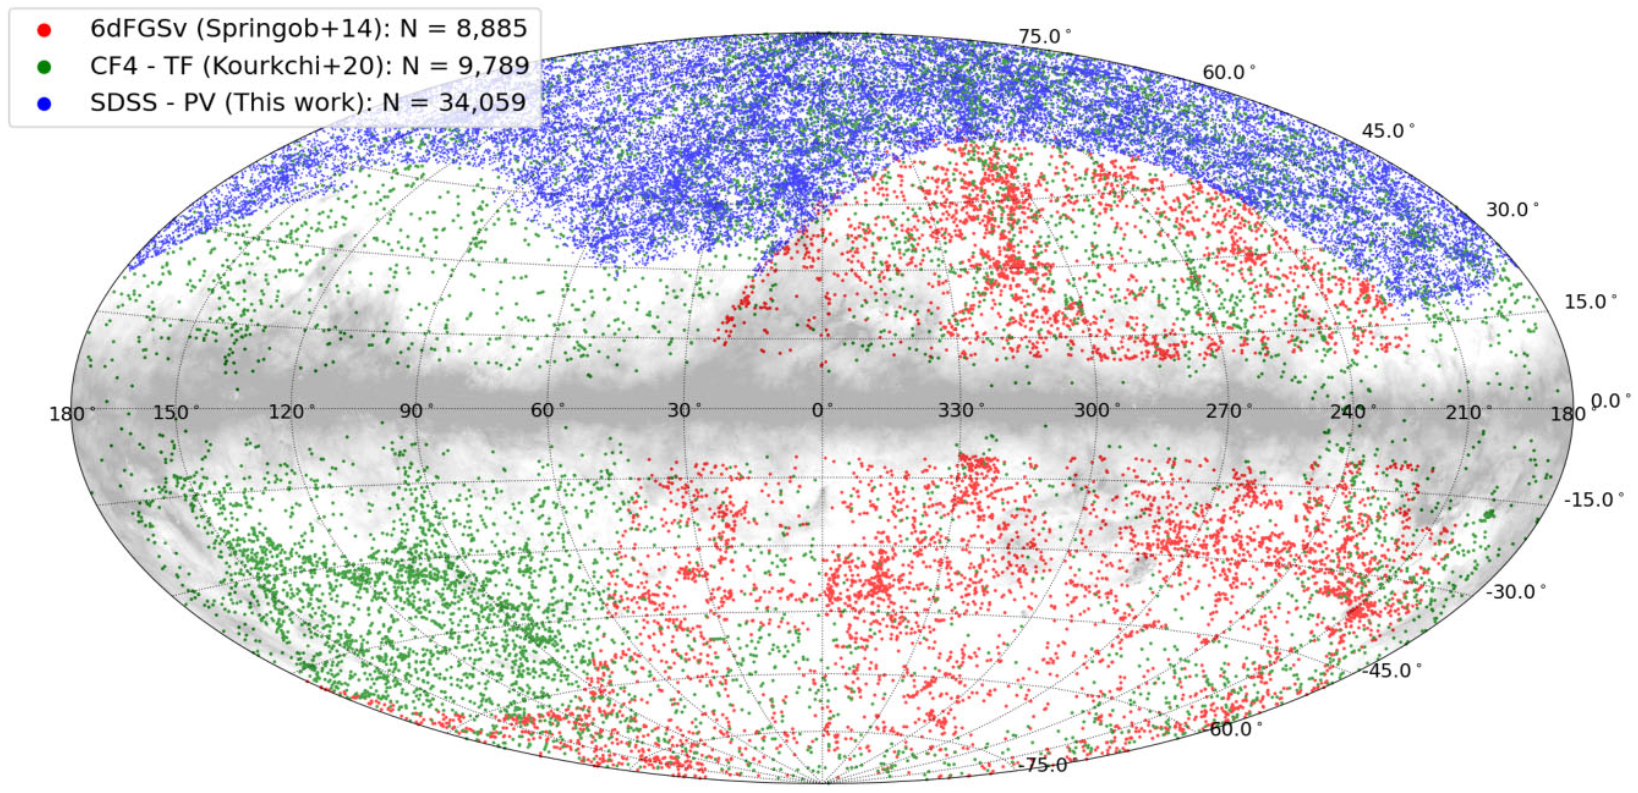
\includegraphics[width=\textwidth]{fig/velocities/pv_footprints.png}
        \caption{Angular distribution of peculiar velocity samples in Galactic coordinates:
        SDSS (blue) and 6dFGSv (red) from Fundamental Plane and 
        Cosmicflows-4 (green) from Tully-Fisher relation.  
        Figure extracted from \cite{howlettSloanDigitalSky2022a}. }
        \label{fig:pv_footprint}
    \end{figure}

    \subsection{The Fundamental Plane of elliptical galaxies} 
    \label{velocities:measuring:fp}
    
    The equivalent of the Tully-Fisher relation for elliptical galaxies is 
    named the Fundamental Plane (FP, \cite{djorgovskiFundamentalPropertiesElliptical1987}). 
    It is an extension in two-dimensions of a previously thought-to-be one-dimensional 
    relation between the luminosity of the elliptical galaxy and 
    the velocity dispersion of their stars near their centres. The one-dimensional version is 
    known as the Faber-Jackson relation (\cite{faberVelocityDispersionsMasstolight1976}). 
    Later, this relation was extended to two-dimensions to relate the effective radius of the galaxy 
    (in kpc) to the velocity dispersion and the average surface brightness within the effective angular radius. 
    The last two quantities are distance-independent and can be observed with spectroscopy and photometry 
    respectively. From these, we can derive the effective radius which is then converted to a distance measurement. 

    The largest sample of FP distances to date is the one produced from the SDSS project 
    (\cite{howlettSloanDigitalSky2022a}) containing about 34~000 distances. 
    This sample recently surpassed the previous larger sample from the 6-degree Field Galaxy Survey 
    peculiar velocity sample (6dFGSv, \cite{springob6dFGalaxySurvey2014}) which contained nearly 9~000 distances. 
    Figure~\ref{fig:pv_footprint} and \ref{fig:pv_zdistrib} show the angular and redshift distribution 
    of these two catalogues, respectively. 
    The final estimated scatter of the SDSS sample is about 50\% in distance moduli 
    which corresponds to about 23\% in distances, which is similar to the scatter of 
    TF distances. 

    In section~\ref{velocities:methods} I will present some of the growth-rate measurements 
    using the 6dFGSv sample of distances. Currently there are no published results using 
    the larger SDSS sample. 

    \begin{figure}[t] 
        \centering 
        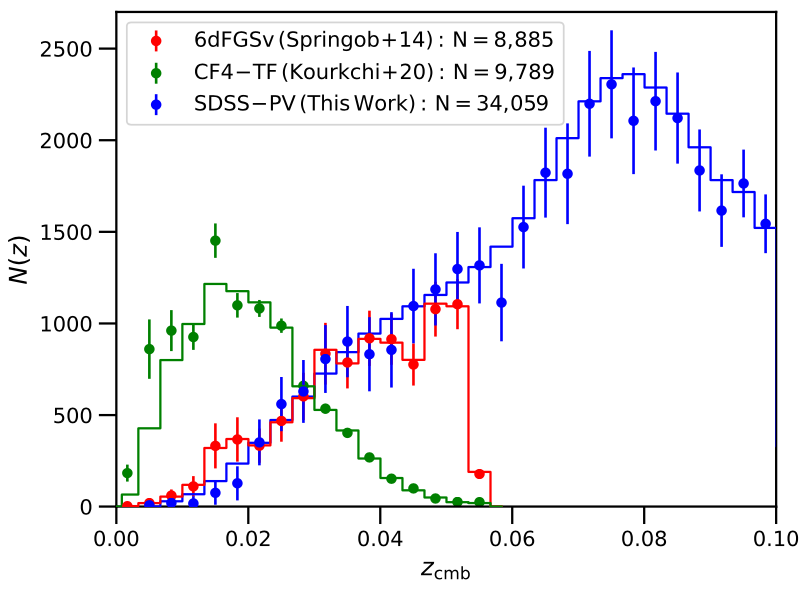
\includegraphics[width=0.5\textwidth]{fig/velocities/pv_zdistrib.png}
        \caption{The redshift distribution of the distance samples: 
        SDSS (blue) and 6dFGSv (red) from Fundamental Plane and 
        Cosmicflows-4 (green) from Tully-Fisher relation. 
        Points with error bars show the number of galaxies per bin of width 1000\kms, 
        where error bars include cosmic variance computed from mock catalogues.
        Solid lines are the mean redshift distributions from these mocks.
        Figure extracted from \cite{howlettSloanDigitalSky2022a}. }
        \label{fig:pv_zdistrib}
    \end{figure}




    \subsection{Type-Ia supernovae}
    \label{velocities:measuring:snia}

    As mentioned earlier, type-Ia supernovae (SNIa) have been used as distance indicators 
    to measure the Hubble constant and the equation of state of dark energy. 
    The state of the art results based on SNIa cover up to redshifts of 2. 

    Since SNIa provide distances, one can also estimate peculiar velocities by 
    looking at the residuals with respect to the best-fit Hubble diagram. 
    Peculiar velocities modifies mostly the observed redshifts than the 
    observed magnitude. Magnitudes are only affected by the relativistic 
    beaming, which scales luminosity distances as $(1+z_\text{pec})^2$, 
    so it is a second-order effect. 
    Figure~\ref{fig:pv_hubble_diagram_snia} sketches how peculiar velocities 
    would impact an ideal case of a SNIa Hubble Diagram without any kind of 
    scatter. We can see how displacements are majoritarily along the redshift direction. 


    \begin{figure}[t]
        \centering 
        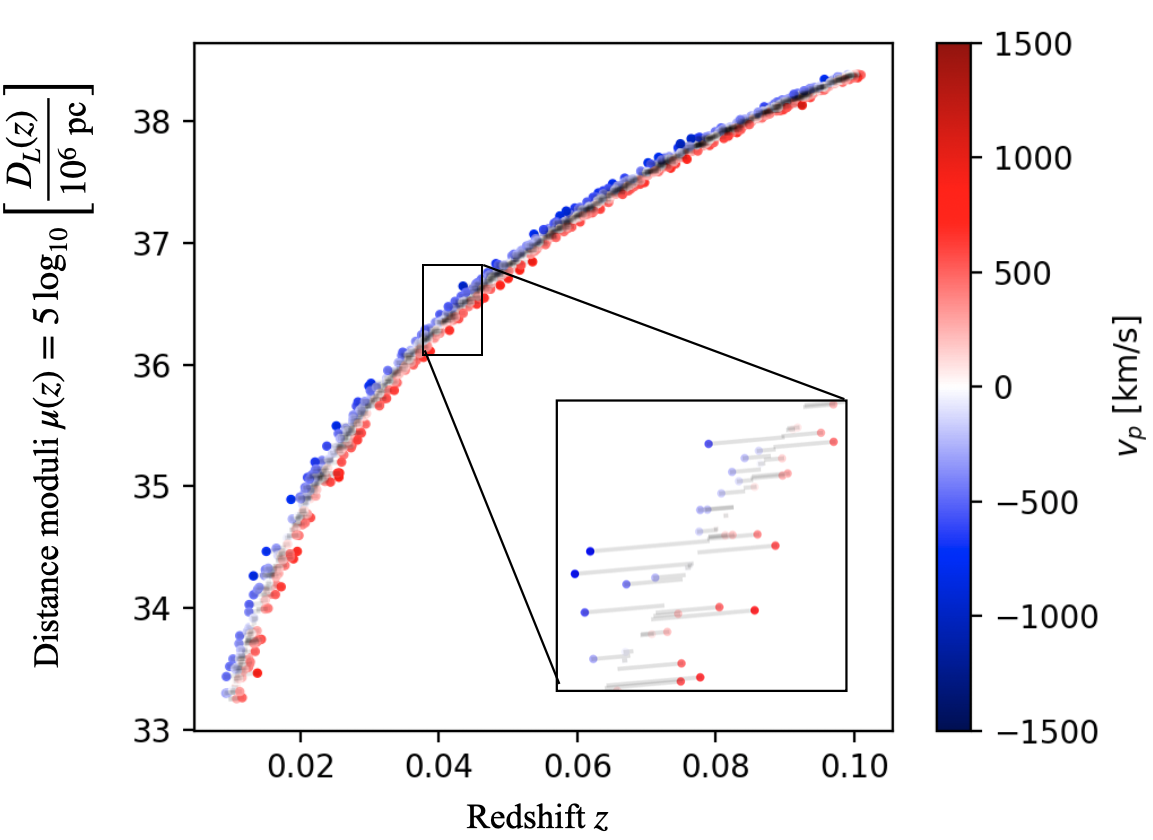
\includegraphics[width=0.7\textwidth]{fig/velocities/pv_hubble_diagram_snia.png}
        \caption{Effect of peculiar velocities on an ideal case of a Hubble Diagram of 
        type-Ia supernovae without any intrinsic scatter or observational uncertainties.
        The displacements along the redshift direction are proportional to $(1+z_\text{pec})$
        while those along the distance moduli direction are proportional to $\log_{10}(1+z_\text{pec})$.
        The colour bar indicates the simulated peculiar velocity of each SNIa. }
        \label{fig:pv_hubble_diagram_snia}
    \end{figure}

    Until now, peculiar velocities were mostly treated as nuisance when 
    constructing the Hubble Diagram. 
    \cite{petersonPantheonAnalysisEvaluating2021} 
    attempted to correct for peculiar velocities of some SNIa of the Pantheon+ sample 
    (\cite{scolnicPantheonAnalysisFull2022}) by using reconstruction techniques on 
    galaxy survey data and by identifying groups of galaxies. 
    Peculiar velocities from SNIa have not been widely used to measure growth-rate for two main 
    reasons. First, the small number of detected SNIa at low redshifts, where uncertainties in 
    velocities are not prohibitive. Second, the inhomogeneity in the available samples which 
    originate from several telescopes, cameras, each with its own observing strategy or 
    prior selection of targets. As we will discuss later, selection effects are important 
    when constructing velocity fields with any type of distance tracer. 
    
    The Zwicky Transient Facility (ZTF, \cite{grahamZwickyTransientFacility2019}) 
    is currently observing the whole available sky from the Northern 
    hemisphere and will produce a large sample of about 5~000 SNIa at $z<0.1$ without any prior 
    selection. This will be a homogeneous set ideal to perform statistical measurements with their 
    peculiar velocities.
    Figure~\ref{fig:pantheon_ztf_sky} compares the angular distribution of SNIa of the Pantheon+ sample 
    to the ZTF Year 1 sample.  
    Figure~\ref{fig:pantheon_ztf_redshift} compares the redshift distribution of the same samples. 
    In section~\ref{velocities:desi_ztf}, I will present the plan of the project of measuring 
    the clustering of ZTF peculiar velocities in combination with galaxies from DESI. 
    
    \begin{figure}[t] 
        \centering 
        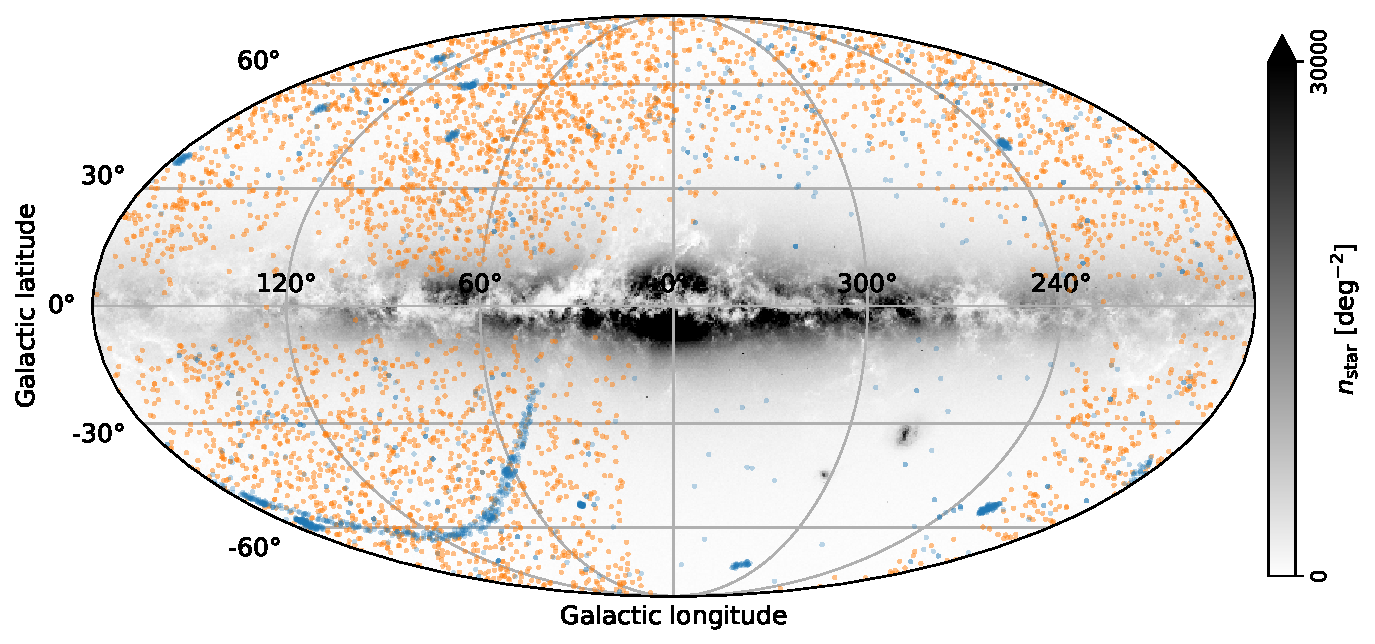
\includegraphics[width=\textwidth]{fig/velocities/ztf_pantheon_gaia.pdf}
        \caption{Angular distribution of type-Ia supernovae in Galactic coordinates
        for the Pantheon+ sample (blue) and for ZTF Year 2 sample (orange). 
        On the background we see the stellar density distribution from Gaia. 
        }
        \label{fig:pantheon_ztf_sky}
    \end{figure}

    \begin{figure}[t] 
        \centering 
        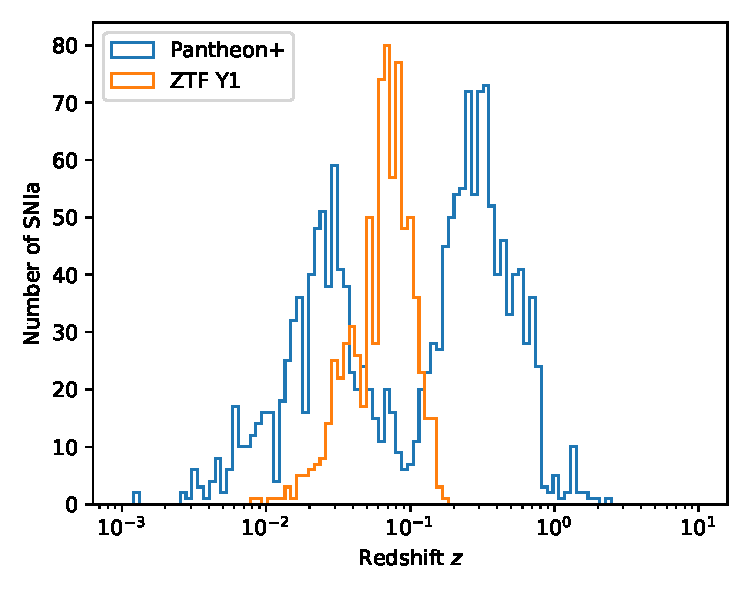
\includegraphics[width=0.6\textwidth]{fig/velocities/nz_ztfy1_pantheon.pdf}
        \caption{Redshift distribution of host galaxies of type-Ia supernovae 
        for the Pantheon+ sample (blue) and for ZTF Year 1 sample (orange).
        }
        \label{fig:pantheon_ztf_redshift}
    \end{figure}

\section{Biases affecting velocities}
\label{velocities:biases}

One of the main difficulties with distance measurements based on standardisable candles 
and their statistical properties (see next section) is the impact of certain types of biases. 
The review by \cite{straussDensityPeculiarVelocity1995} discuss all these biases and how they  
impact clustering analyses. They can be classified in three types: selection bias, homogeneous 
and inhomogeneous Malmquist biases. The term Malmquist is often used to refer to selection bias,
but I will follow the convention of \cite{straussDensityPeculiarVelocity1995}. 

The selection bias, as the name indicates, is caused by some selection or detection criteria 
on the sample of objects. For instance, it is pretty common to impose some cuts on signal-to-noise 
ratio of fluxes or some magnitude limit. For objects close to the boundary, only 
the brighter objects pass the cuts. If one is interested in, say, the average distance of these objects, 
we will observe a bias relative to the true average distance. 
The intrinsic scatter in luminosity of all standardisable candles worsens this type of bias 
and it complicates any attempts to correct for these biases. 
Typical analyses of SNIa often use realistic simulations of the data, including the physical 
properties of SNIa that create the scatter and instrumental noise, to model these selection effects. 
The analysis of the Pantheon SNIa sample used a technique named 
Bayesian Estimation Applied to Multiple Species (BEAMS, \cite{kunzBayesianEstimationApplied2007}) 
with Bias Corrections 
(BBC, \cite{kesslerCorrectingTypeIa2017}). This technique also accounts for mis-classified supernovae. 

The homogeneous Malmquist bias manifests itself due to the fact that the number of objects 
observed as a function of distance to us increases with distance squared. When averaging 
objects in a given distance or redshift range, they are not uniformly distributed inside this range,
so the average distance is higher than the true distance, often assigned to the center of the range. 
Is this true ? Check! 
 
The inhomogeneous Malmquist bias is a similar effect but generalised to the fluctuations in density 
(due to structures) along the line of sight. This bias depends on the precise shape of $\delta(\hat{n}, d)$
where $\hat{n}$ is a given direction in the sky and $d$ is the distance to us. 

It is possible to correctly account for all these biases in a fully Bayesian treatment of  
probability density functions of the distances 
(\cite{grazianiPeculiarVelocityField2019, boruahReconstructingDarkMatter2021}). 

\section{Growth-rate measurements with velocities}
\label{velocities:methods}


With a set of distance or peculiar velocity measurements, 
we can study them statistically and compare to predictions from 
cosmological models, just as we did with the overdensities of fluxes 
in chapter~\ref{chap:forests} or galaxies in chapter~\ref{chap:galaxies}. 

One can see this additional set of observables as a scalar field, the radial 
velocity field  $v_r(\vec{x}_i)$, sampled 
at the positions of the galaxies from which they were measured $\vec{x}_i$, 
where $i=1,\ldots,N_\text{gal}$. 
Instead of radial velocities, it is quite common to use the log of the ratio between the distance inferred from 
the redshift and the distance inferred from the luminosity, called log-distance ratio. 
Log-distance ratios have uncertainties that can be approximated by a Gaussian, 
whereas in velocity space the uncertainties become log-normal are harder to handle. 

The first statistic that one can think of measuring is the correlation function of the 
radial velocities  $\xi_{v_r v_r} \equiv \langle v_r(\vec{x}_i) v_r(\vec{x}_j) \rangle$ 
(or the equivalent for log-distance ratios). 
If one has, in addition to the velocities, a galaxy survey over the same volume, one
can use the observed overdensity field $\delta(\vec{x})$ to cross-correlate with the 
observed velocity field, i.e., $\xi_{\delta_g v_r} \equiv \langle \delta(\vec{x}) v_r(\vec{y})\rangle$. 
The auto-correlation of the overdensity field $\xi_{\delta_g \delta_g} \langle \delta(\vec{x})\delta(\vec{y})\rangle$ 
is the equivalent to the one used in BAO and RSD measurements. 
These three statistics can be analysed jointly when comparing to models, 
increasing the constraining power. 

I will shortly describe a few methods available in the literature that 
allows us to connect models to the observed densities and velocities, 
at the field level or at the two-point function level. 

    \subsection{Maximum likelihood method}
    \label{velocities:methods:maximum_likelihood}

    The idea is to maximise the likelihood, assumed to be a multivariate Gaussian on 
    the velocities,
    \begin{equation}
        \mathcal{L}(\vec{p}) = \frac{1}{(2 \pi)^{\frac{n}{2}} \text{det}[C(\vec{p})]^{1/2} }
            \exp\left[-\frac{1}{2} v_r^T C(\vec{p})^{-1} v_r\right]
        \label{eq:likelihood}
    \end{equation}

    with respect to a set of parameters $\vec{p}$. Here $v_r$ is a vector containing each 
    measured peculiar velocity and the covariance matrix $C(\vec{p})$ is the model 
    for the two-point statistics of $v_r$. Each element of the covariance is given by 
    $C_{ij} =  \xi^\text{model}_{v_r v_r}(\vec{x}_i, \vec{x}_j, \vec{p}) + \delta^K_{ij} \sigma_i \sigma_j$, 
    where $\sigma_i$ is a diagonal noise term, often accounting for instrumental uncertainties 
    as well as intrinsic scatter of distance measurements. 
    The first term in the covariance 
    is the cosmic variance and it is connected to a cosmological model. 

    The cosmological part of the covariance $C_{ij}$ is often written as a 
    Fourier transform of the two-point statistics in Fourier space, 
    often described by the velocity or the velocity-divergence power 
    spectrum. 
    Most of previous works have used linear perturbation theory with  
    some empirical terms that account for non-linearities.  
    In linear theory, the velocity field $\vec{v}(\vec{x})$ is irrotational, meaning it 
    is completely defined as the gradient of a scalar field $\theta(\vec{x})$. 
    This velocity divergence is equal to the overdensity of matter $\delta(\vec{x})$ for linear perturbations. 
    Therefore the two-point statistics of the velocity is proportional to the linear matter power spectrum 
    (and thus to $\sigma^2_8$) and to the linear growth-rate of structures $f$. 

    The maximum likelihood method has been used on several peculiar velocity samples
    such as the 6dFGSv (\cite{campbell6dFGalaxySurvey2014, springob6dFGalaxySurvey2014})
    with velocities alone (\cite{johnson6dFGalaxySurvey2014}), in combination with density field 
    (\cite{adamsImprovingConstraintsGrowth2017, adamsJointGrowthrateMeasurements2020}), 
    or adding a few SNIa (\cite{hutererTestingLCDMLowest2017}). 
    
    At CPPM, Bastien Carreres is currently employing this technique to analyse 
    the ZTF sample of type-Ia supernovae. I have implemented the basic algorithm 
    and Bastien continued its development, adapting it to work with log-distance 
    ratio instead of velocities, several mesh assignment schemes and models of clustering. 
    He also implemented a whole pipeline to produce realistic simulations of ZTF SNIa light-curves, 
    which can be painted on n-body simulations, and to analyse them as real data. 
    He is currently studying 
    the impact of selection biases on the estimates of $f\sigma_8$ using the 
    maximum likelihood method. First results on simulated data show that an unbiased measurement 
    is possible if we limit our analysis to SNIa at $z< 0.05$. 
    We will apply our methodology to real data once the final ZTF SNIa is set. 


    \subsection{Compressed two-point statistics}
    \label{velocities:methods:compressed_two_point} 

    The compression of two-point statistics means that we combine measurements 
    into separation or wavenumber bins, depending if we are in configuration or Fourier space. 
    Estimating compressed statistics is the most common method for  
    standard clustering analysis, as we saw in earlier chapters, 
    where we aim to estimate the correlation function or the power spectrum.
    The modelling happens at the compressed statistics level, so there are generally less 
    degrees of freedom than for the maximum likelihood method. 

    In configuration space, the velocity auto correlation cannot simply be written as 
    a unique function of separation $\vec{r}$ between two galaxies, since velocities are 
    a vector field. \cite{gorskiPatternPerturbationsHubble1988} introduced the 
    correlation tensor defined as 
    \begin{equation}
        \Psi_{i, j}(\vec{r}_A, \vec{r}_B) \equiv \langle v_i(\vec{r}_A) v_j(\vec{r}_B) \rangle 
        \label{eq:correlation_tensor}
    \end{equation}
    where $i, j$ denote each component of the peculiar velocity field $\vec{v}$. 
    If the field is irrotational, homogeneous and isotropic, the correlation tensor 
    can be written as 
    \begin{equation}
        \Psi_{i, j}(\vec{r}) = 
        \left[ \Psi_\parallel(r) - \Psi_\perp(r) \right] \hat{r}_{Ai} \hat{r}_{Bj} 
        + \Psi_\perp(r) \delta^K_{ij}
    \end{equation}
    where $\Psi_\parallel(r)$ and $\Psi_\perp(r)$ are functions describing the correlations 
    the components of the peculiar velocities parallel and perpendicular to the 
    separation vector $\vec{r}$. Both functions can be written as transforms of the linear 
    matter power spectrum. 

    The correlations between the radial velocities of two galaxies
    relative to the observer, as depicted in 
    Figure~\ref{fig:pv_config}, can be written as 
    \begin{equation}
        \langle u_A(\vec{x})u_B(\vec{x}+\vec{r}) \rangle = 
        \Psi(r) \cos \theta_{AB} 
        + \left[ \Psi_\parallel(r) - \Psi_\perp(r) \right] \cos \theta_A \cos \theta_B. 
    \end{equation}
    
    

    \begin{figure}[t]
        \centering 
        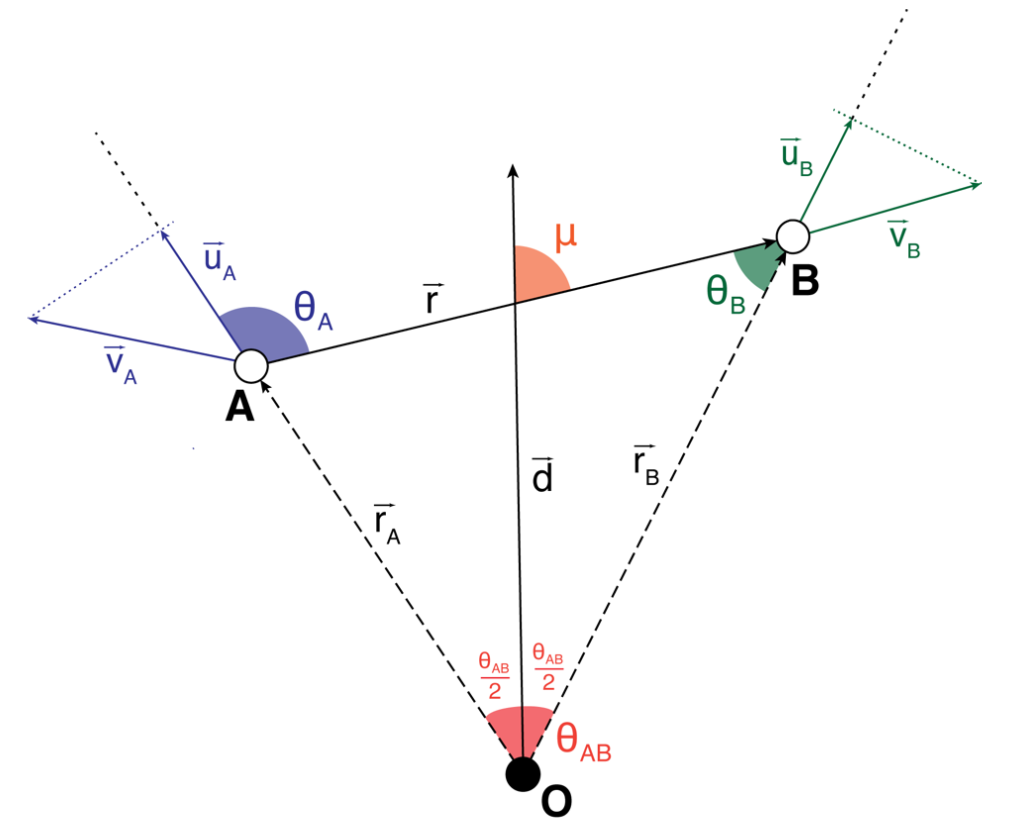
\includegraphics[width=0.6\textwidth]{fig/velocities/pv_config.png}
        \caption{Non-parallel lines-of-sight of a pair of galaxies A and B as seen by an observer O.
        $\vec{r}_A$ and $\vec{r}_B$ are their position vectors, respectively, 
        and $\vec{r}$ is the separation vector between them. 
        The peculiar velocities of galaxies A and B are represented by $\vec{v}_A$ and $\vec{v}_B$, 
        and the radial component of these velocities are represented by $\vec{u}_A$ and $\vec{u}_B$. 
        The pair line-of-sight $\vec{d}$ is defined at the mid-angle and $\mu \equiv \hat{d} \cdot \hat{r}$. 
        Figure extracted from \cite{turnerLocalMeasurementGrowth2023}. 
        }
        \label{fig:pv_config}
    \end{figure}

    \cite{gorskiCosmologicalVelocityCorrelations1989} developed estimators that we can 
    relate to a model that depends on $\Psi_\parallel$ and $\Psi_\perp$. 
    This type of correlation functions were used in 
    \cite{wangPeculiarVelocityCorrelation2018, 
    dupuyEstimationLocalGrowth2019, 
    turnerImprovingEstimatesGrowth2021,
    turnerLocalMeasurementGrowth2023}. 

    In Fourier space, given the sparsity of the data, it is hard to use FFTs on the 
    observed velocity field. This is because voxels without data cannot be assigned 
    zero velocity: the field would be ill-defined there. 
    For this reason, 
    \cite{howlettRedshiftspaceMomentumPower2019} suggests to use the momentum power 
    spectrum, a quantity commonly used in the analysis of velocities in n-body simulations. 
    The momentum is simply the mass-weighted velocity field, written as
    $\vec{p}(\vec{x}) = \left[1+\delta(\vec{x})\right] \vec{v}(\vec{x})$. 
    In the absence of galaxies or velocity measurements, 
    the momentum is well defined and equal to zero. 

    The first application of the momentum power spectrum method was 
    performed by \cite{qinRedshiftspaceMomentumPower2019} on the combined 
    sample of 6dFGSv and the 2MASS Tully-Fisher survey (2MTF). 

    The analysis in compressed statistics is generally faster and more intuitive
    than other methods. The data versus model comparison is commonly easier with 
    compressed statistics. However, one has to be careful when accounting for 
    survey properties, wide-angle effects or redshift evolution. These effects
    are generally easier to deal with in other methods. 


    \subsection{Density-velocity comparison}
    \label{velocities:methods:comparison}

    The link between density and velocity fields is straightforward 
    on quite large scales, where linear theory is valid. 
    Another method to test for the consistency of the standard cosmological model 
    is to compare the observed (radial) velocity field with 
    predictions based on the observed density field. 
    This method is often referred to as density-velocity comparison.  

    Reconstruction techniques discussed in section~\ref{galaxies:reconstruction}
    aim to compute past trajectories of galaxies and therefore their velocities based 
    on the observed density field. Reconstruction yields a prediction for the radial 
    velocities at the locations where we measured them from the distance surveys.
    The inputs are often some value for the large scale bias $b$ of the galaxy sample 
    as well as the growth-rate $f$.  
    Commonly, an empirical amplitude $A$ is fitted to the relation $v_r^\text{obs} = A v_r^\text{model}$. 
    Any deviations from $A=1$ would indicate an inconsistency in the standard 
    cosmological model. From this amplitude, one can quote a value for $f\sigma_8$ 
    if a bias value and a $\sigma_8$ value are assumed.  

    Several applications of this method can be found in he literature. 
    \cite{davisLocalGravityLocal2011} used the Two Micron All-Sky Redshift Survey 
    (2MRS or 2M++ for its extended version) 
    galaxy catalogue as the input for reconstruction and fitted 
    the inverse Tully-Fisher relation to spiral galaxies from the 
    Spiral Field I-band ++ survey (SFI++). 
    \cite{carrickCosmologicalParametersComparison2015} improved the analysis 
    and reported results using the same samples. 
    \cite{boruahCosmicFlowsNearby2020} added peculiar velocities from 465 SNIa 
    to the SFI++ and the 2MTF samples. 
    \cite{saidJointAnalysis6dFGS2020} used a larger dataset of nearly 16k peculiar velocities 
    by combining 6dFGSv and SDSS samples, and compared to the density field from the 2M++. 
    
    At CPPM, Elena Sarpa has a more advanced reconstruction technique 
    called extended Fast Action Minimization (eFAM, \cite{sarpaExtendedFastAction2021})
    which can be readily used to implement the density-velocity comparison.
    The eFAM technique yields higher-order trajectories than 
    Zeldovich reconstruction, which might lead to more realistic 
    predictions for the peculiar velocities. 
    This technique will be potentially applied to the DESI and ZTF data,
    after a detailed comparison with the maximum likelihood method. 


    \subsection{Forward-model of density and velocity field}
    \label{velocities:methods:forward}

    Instead of estimating summary statistics with the density and velocity fields, 
    one can attempt to fit directly the observed fields with some model 
    that depend on cosmological parameters. Typically, the model is composed 
    of some cosmological parameters and a set of initial density and velocity fields
    (one amplitude parameter per mode). These initial conditions are then evolved 
    linearly or using more advanced techniques and then compared to observations. 
    The final product is a posterior on cosmological parameters and on the amplitudes 
    of the initial fields. This method is commonly referred to as \emph{forward-modelling}. 

    In forward modelling, complications due to selection functions are slightly easier 
    to deal with in principle. One has to simulate observations on the evolved fields j
    ust as one does when creating mock catalogues. 
    Also, by modelling the observed field entirely, we capture 
    more information from higher-order statistics than just the two-point function. 
    The inconvenience of this method is the computing time required to perform the inference,
    given the large number of free parameters and the time to evolve each sample from initial conditions. 
    
    \cite{lavauxBayesian3DVelocity2016} implemented the forward-modelling applied to 
    both density and velocity fields. A similar approach was used on CosmicFlows3 data 
    by \cite{grazianiPeculiarVelocityField2019}. In \cite{boruahReconstructingDarkMatter2021}
    they discuss the treatment of the inhomogeneous Malmquist bias in the Bayesian formalism 
    (see section~\ref{velocities:biases}).
    In \cite{prideaux-gheeFieldbasedPhysicalInference2023}, they used a Bayesian hierarchical modelling 
    approach to fit both density and velocity fields using a Hamiltonian Monte Carlo sampling of the 
    likelihood. 

\section{Current measurements}
\label{velocities:current}

Several measurements were made in the past decade using a variety of distance surveys, 
galaxy surveys and methods. 
Table~\ref{tab:pv_current_measurements} summarises most measurements in the literature.
They are also visually represented in Figure~\ref{fig:pv_current_measurements}. 
All these measurements of the growth-rate $f\sigma_8$ correspond to an effective redshift between zero and 0.1. 
These results are in good agreement with the predictions from a $\Lambda$CDM+GR model, with 
cosmological parameters from \cite{planckcollaborationPlanck2018Results2020}. 
However, one can notice how they do not have the same uncertainties, even if, for some cases, they 
use the same datasets. Few analyses quote systematic uncertainties which can be quite significant for  
some methods. 

The goal of the project I am currently leading at CPPM is to deeply understand those variations 
while optimising the analysis. Also we plan to work closely to the data reduction teams 
in order to produce the best set of simulated data. 
Mock catalogues will be essential to estimate biases 
in best-fit parameters, statistical and systematic uncertainties. 
In the following section I will introduce two datasets that will be used in our project: DESI and ZTF. 

\begin{table}
    \small 
    \centering
    \caption{Measurements of the growth-rate of structures from peculiar velocity 
    and galaxy survey data. }
    \label{tab:pv_current_measurements}
    \begin{tabular}{lllc} 
        \hline 
        \hline 
        Reference  &  Dataset  &  Method   &   $f\sigma_8$  \\ 
        \hline 
%\cite{beutler6dFGalaxySurvey2012a}          & 6dFGSz    & RSD               & $ 0.423 \pm 0.055 $           \\
%\cite{blakePowerSpectrumMultipoles2018}     & 6dFGSz    & RSD               & $ 0.380 \pm 0.120 $ \\
\cite{johnson6dFGalaxySurvey2014}           & 6dFGSv    & Max-likelihood    & $ 0.428^{+0.079}_{-0.068} $   \\
\cite{hutererTestingLCDMLowest2017}         & 6dFGSv    & Max-likelihood    & $ 0.428^{+0.048}_{-0.045} $   \\
\cite{adamsJointGrowthrateMeasurements2020} & 6dFGSz,6dFGSv & Max-likelihood & $ 0.384 \pm 0.052^\text{(stat)} \pm 0.061^\text{(syst)} $ \\  
\cite{laiUsingPeculiarVelocity2023}        & SDSS-FP   & Max-likelihood    & $ 0.405^{+0.076 \text{(stat)}}_{-0.071} \pm 0.009^\text{(syst)} $ \\
\cite{qinRedshiftspaceMomentumPower2019}    & 6dFGSv,2MTF & Compressed 2pt  & $ 0.404^{+0.082}_{-0.081} $ \\
\cite{howlett2MTFVIMeasuring2017}           & 2MTF      & Compressed 2pt    & $ 0.510^{+0.090}_{-0.080} $ \\
\cite{nusserVelocitydensityCorrelationsCosmicflows32017} 
                                            & CF3,2MRS  & Compressed 2pt    & $  0.400 \pm 0.080 $ \\ 
\cite{dupuyEstimationLocalGrowth2019}       & CF3       & Compressed 2pt    & $ 0.430 \pm 0.030^\text{obs} \pm 0.110^\text{cosmic} $ \\ 
\cite{davisLocalGravityLocal2011}           & 2MRS,SFI++ & $\delta-v$ comparison & $ 0.310 \pm 0.040 $ \\
\cite{carrickCosmologicalParametersComparison2015} 
                                            & 2MRS,SFI++ & $\delta-v$ comparison & $ 0.401 \pm 0.024 $ \\
\cite{boruahCosmicFlowsNearby2020}          & 2M++,2MTF,SFI++,A2 &  $\delta-v$ comparison & $ 0.400 \pm 0.017 $ \\
\cite{saidJointAnalysis6dFGS2020}           & 2M++,6dFGSv,SDSS-FP & $\delta-v$ comparison & $ 0.311 \pm 0.027 $ \\

        \hline 
        \hline 
    \end{tabular}
\end{table}

\begin{figure}[t]
    \centering 
    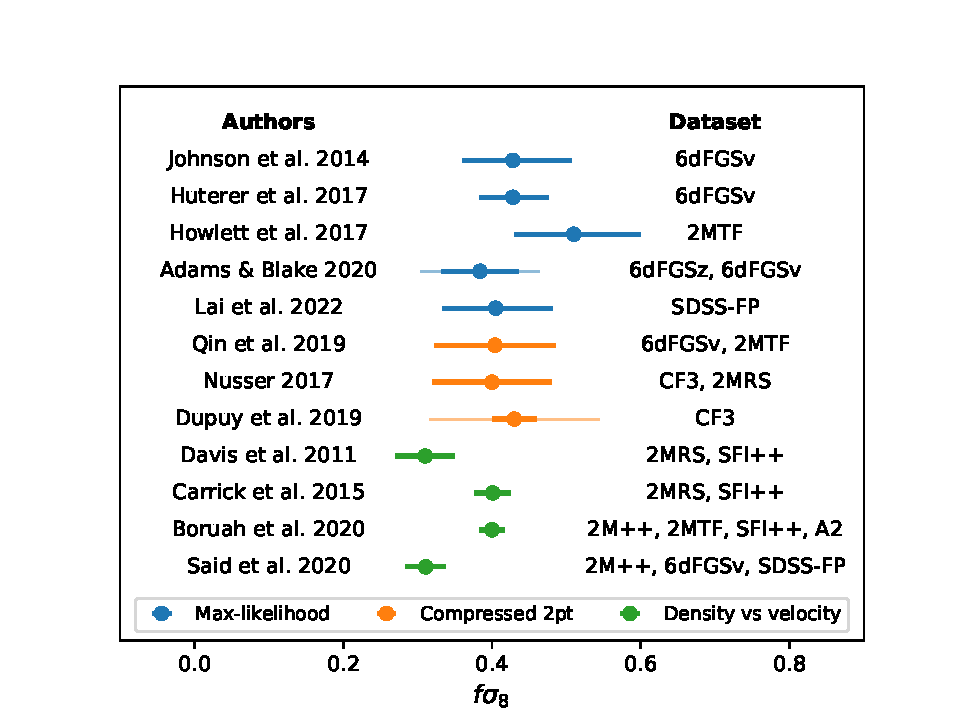
\includegraphics[width=0.8\textwidth]{fig/velocities/plot_fs8_pv.pdf}
    \caption{Measurements of the growth-rate of structures $f\sigma_8$ from peculiar velocity 
    and galaxy survey data. The references and values are listed in Table~\ref{tab:pv_current_measurements}.
    The light error bars include systematic errors. In the case of Dupuy et al. 2019, the extra contribution 
    is from cosmic variance, instead. }
    \label{fig:pv_current_measurements}
\end{figure}

\section{DESI and ZTF}
\label{velocities:desi_ztf}

Both the Dark Energy Spectroscopic Instrument (DESI) and the Zwicky Transient Facility (ZTF)
are currently observing similar area of the sky and building one of the best samples for a joint study of 
densities and peculiar velocities for cosmology. 
One of the main advantages is the great overlap in volume of both surveys. The 14k deg$^2$ footprint 
of DESI will be completely covered bt ZTF observations, which cover up to 18k deg$^2$ of area. 

The main science goal of DESI is to produce precise measurements of the Universe's expansion and 
the growth history of structures, in order to test models of dark energy and gravity. 
DESI will observe more than 20 million galaxies and quasars from up to redshifts of 4.5. 
The bright time of the survey, i.e., when the moon is up, is dedicated to building a flux limited sample of
galaxies at low redshift: the Bright Galaxy Survey (BGS). The BGS will collect roughly 10 million galaxies 
with $r$-band magnitude $r < 19.5$, which lie at $z < 0.6$. 
A fainter  $19.5<r<20.175$ sample will extend and increase the completeness in stellar mass of the BGS sample. 
This sample is not only ideal for BAO and standard RSD measurements, but also for higher order statistical 
measurements, multi-tracer analyses, given its high completeness and simple selection function. 
Most of the ZTF SNIa will have their host-galaxy redshifts measured by the DESI BGS.
It is expected that the BGS observations will complete by 2024 the latest. 

The ZTF survey main goal is to observe the transient sky in three optical bands. 
Most of the sky area is covered every two nights with a given filter, which is excellent cadence 
for discovery and study of SNIa. 
At its current configuration, ZTF is expected to discover around 15k supernovae, 
out of which about 30\% will have spectroscopic classifications. 
The host galaxy redshifts are obtained from archival data, some of which will be observed by DESI 
in the near future. We expect a final sample of 5k cosmology-level spectroscopic SNIa at  
$z < 0.1$. 

Figure~\ref{fig:nz_desi_ztf} compares the density of tracers between DESI BGS and ZTF SNIa, expected at 
the end of their 5-year programs. The density of ZTF SNIa falls quickly after $z \sim 0.06$ where 
selection effects start to kick in. Rough estimates show that the ZTF SNIa sample is \emph{complete},
i.e., all potentially observable SNIa were observed, at $z < 0.05$. 
While the density of ZTF SNIa is several orders of magnitudes lower 
than those of BGS galaxies, the fact that each SNIa yields a measurement of the velocity field 
makes them a powerful tracer nevertheless. 

\begin{figure}[t]
    \centering
    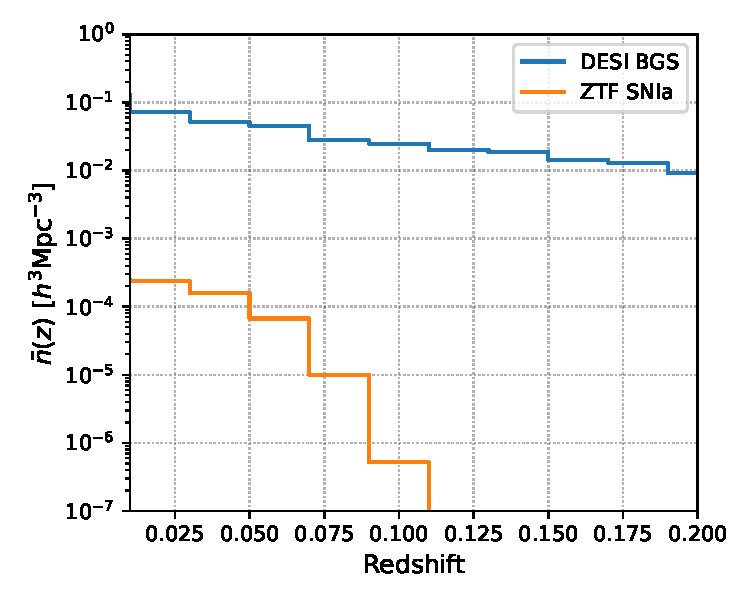
\includegraphics[width=0.5\textwidth]{fig/velocities/nz_desi_ztf.pdf}
    \caption{Comoving density of tracers as a function of redshift for the galaxies of 
    the DESI Bright Galaxy Survey (blue) and for type-Ia supernovae from ZTF (orange).
    Densities were computed assuming a flat $\Lambda$CDM model with 
    Planck 2018 best-fit parameters, based on simulated data and scaled to 
    match numbers expected at the end of both programs. 
    Both samples overlap in redshift and in sky coverage, which is ideal for joint studies 
    of densities and peculiar velocities. 
    }
    \label{fig:nz_desi_ztf}
\end{figure}


I studied the constraining power of DESI BGS and ZTF SNIa using the Fisher formalism.
I computed the uncertainty expected on $f\sigma_8$ from a RSD analysis with DESI BGS galaxies by themselves  
or from a joint RSD + PV analysis of DESI BGS and ZTF SNIa. 
I employed the same Fisher forecast code\footnote{\url{https://github.com/CullanHowlett/PV_fisher}} 
described in \cite{howlettMeasuringGrowthRate2017}. 
The inputs of the calculation are the expected comoving density of tracers for galaxies and peculiar velocities
at the end of both surveys, 
the intrinsic scatter of the distance indicators parametrised by $\alpha \equiv \sigma(D_L)/D_L \sim $10 or 20\%, 
and the scale range (in Fourier space) assumed for the measurement parametrised by $k_\text{max} \sim 0.1$ or $0.2~h\text{Mpc}^{-1}$. 
The model for the galaxy clustering is a simple linear RSD model with galaxy bias $b$ and 
a Gaussian Fingers-of-God term function of a galaxy velocity dispersion $\sigma_v$. 
The model for the velocity correlations is similar, scaling with $f$, but with a different 
empirical correction for the fact we observe velocities in redshift-space  (\cite{kodaArePeculiarVelocity2014}).
This empirical function depends on an extra dispersion parameter $\sigma_u$. 
A total of four free parameters define the model. I focused on the constraints on $f\sigma_8$ 
by using tracers over $0< z < 0.1$, which corresponds to a measurement at an effective 
redshift $z_\text{eff} = 0.08$. 

Results of the Fisher forecast are shown in Table~\ref{tab:forecast_fs8}
for different samples and analysis choices. 
First, we can see how the uncertainties on $f\sigma_8$ are 
significantly reduced when including ZTF SNIa, particularly when 
the intrinsic scatter is small and when using a larger range of scales. 
We see an improvement of a factor of 2.3 at most.  
Second, we see how increasing the scale range $k_\text{max}$ also improves constraints. 
This is why it is important to be able to model the clustering of galaxies and 
peculiar velocities on non-linear scales. 
Third, we see how improving the standardisation of SNIa also helps 
reducing uncertainties on $f\sigma_8$. 
In conclusion, a simple Fisher forecast predicts a 9\% measurement of $f\sigma_8$ 
in the optimistic scenario and a 20\% in the pessimistic scenario. 

\begin{table}
    \centering 
    \caption{Fisher forecast on measurements of the growth-rate of structures times the normalisation of the power spectrum 
    $f\sigma_8(z_\text{eff}) = 0.45$ where $z_\text{eff} = 0.08$ for the complete samples of DESI BGS and ZTF type-Ia supernovae. 
    Results are shown for different analysis choices: $k_\text{max}$ is the maximum wavenumber used in the analysis, 
    $\sigma(D_L)/D_L$ is the fractional error on luminosity distances due to intrinsic scatter. 
    The assumed number densities of tracers is the one shown in Figure~\ref{fig:nz_desi_ztf}. 
    The total assumed sky area with overlapping coverage from both experiments is 14k deg$^2$.
    }
    \label{tab:forecast_fs8}
    \begin{tabular}{lccc}
\hline 
\hline 
Dataset   & $k_\text{max}$  &  $\sigma(D_L)/D_L$  &     $\sigma \left(f\sigma_8(z_\text{eff})\right)/f\sigma_8(z_\text{eff})$ \\ 
\hline
DESI BGS  &  0.1 &  - &  0.58 \\
DESI BGS  &  0.2 &  - &  0.21 \\
ZTF SNIa  &  0.1 &  0.05 &  0.22 \\
ZTF SNIa  &  0.1 &  0.10 &  0.35 \\
ZTF SNIa  &  0.2 &  0.05 &  0.19 \\
ZTF SNIa  &  0.2 &  0.10 &  0.32 \\
DESI BGS + ZTF SNIa  &  0.1 &  0.05 &  0.12 \\
DESI BGS + ZTF SNIa  &  0.1 &  0.10 &  0.20 \\
DESI BGS + ZTF SNIa  &  0.2 &  0.05 &  0.09 \\
DESI BGS + ZTF SNIa  &  0.2 &  0.10 &  0.13 \\
\hline
\hline
    \end{tabular}
\end{table}


\section{Growth-rate measurement from simulated ZTF data}
\label{velocities:ztf_fs8}

Bastien Carreres, PhD student I co-supervise with Benjamin Racine and Dominique Fouchez at CPPM, 
is currently developing the whole analysis chain to measure the growth-rate of structures 
from peculiar velocities derived from ZTF type-Ia supernovae (SNIa) data. 
He has been developing a code based on the maximum-likelihood method 
(section~\ref{velocities:methods:maximum_likelihood}) and validating it with 
the most realistic set of simulated ZTF data that he also produced. 
In this section, I summarise his findings which will be detailed in 
Carreres et al. (in prep). 

\subsection{Simulating ZTF type-Ia supernovae with peculiar velocities}
\label{velocities:ztf_fs8:sims}

The goal of the simulations is to create a set of light-curves from SNIa 
which contain realistic and correlated peculiar velocities. 

The best source of peculiar velocities are n-body simulations. 
We currently use two sets of large-scale cosmological n-body simulations 
with matter only. The first set is named Dark Energy and Massive Neutrino Universe 
(DEMNUni, \cite{castorinaDEMNUniClusteringLargescale2015}) aimed at account correctly for 
the impact of massive neutrinos in the formation of structures. 
They were produced with the tree particle mesh-smoothed particle hydrodynamics 
(TreePM-SPH) code Gadget-3 with a recipe given by \cite{vielEffectNeutrinosMatter2010} 
to simulate massive neutrinos. The DEMNUni boxes are 2 $h^{-1}$Gpc on a side, 
and contain 2048$^3$ matter particles and $2048^3$ neutrino particles. Initial conditions 
are set at $z=99$ and evolved assuming a flat $\Lambda$CDM universe with parameters 
from Planck 2013 results (\cite{planckcollaborationPlanck2013Results2014a}). 
Different simulations were ran with varying mass of neutrino species (0, 0.16, 0.32, and 0.48 eV)
and varying equations-of-state for dark energy. 
Haloes were defined using a Friend-of-friends algorithm, assembling a minimum number of 32 
matter particles. This first set of simulations is not yet public and access it only granted 
by demand to the authors. 
The second set of simulations we use are the AbacusSummit suite (\cite{maksimovaABACUSSUMMITMassiveSet2021}), 
which use the Abacus code (\cite{garrisonABACUSCosmologicalNbody2021}) to produce 
150 boxes of 2 $h^{-1}$Gpc on a side, containing 6912$^3$ particles and 
spanning 97 cosmological models. These cosmological models have different 
values for $\omega_b$, $\omega_\text{cdm}$, $h$, $A_s$, $n_s$, $\alpha_s$, 
$N_\text{eff}$, $w_0$ and $w_a$. Initial conditions are created using 
first order Lagrangian perturbation theory with the public code
\textsc{Zeldovich-PLT}\footnote{\url{https://github.com/abacusorg/zeldovich-PLT}}.
Halos are found using the CompaSO technique (\cite{hadzhiyskaCOMPASONewHalo2022}).
These simulations and several data products are publicly available and 
documented\footnote{\url{https://abacussummit.readthedocs.io/}}. 
The AbacusSummit suite is currently the state-of-the-art in the market 
and are currently being used by the DESI collaboration. 

ZTF observes spectroscopically classified SNIa 
up to redshifts of 0.1, which corresponds to a comoving distance 
of $\sim 293$\hmpc in a Planck 2018 best-fit cosmology. 
This means that we can subdivide a $(2~h^{-1}\text{Gpc})^3$ simulation box into 
roughly 9 ZTF SNIa volumes (full-sky, even though ZTF observes the Northern sky).  
Because of large-scale correlations, these sub-boxes are not completely independent of each other. 
We place the observer at the center of each sub-box and compute the radial 
component of peculiar velocities for each halo. 
Eventually we convert comoving distances into redshifts assuming a fiducial cosmology. 
At this step, we can also include the effect of redshift-space distortions (RSD) using the radial velocities.
Currently we do not apply any halo mass cuts in our halo samples. 

With halo samples in hand, we randomly assign SNIa events following a given rate of 
events per volume, e.g., $(2.35 \pm 0.24) \times 10^4 \text{Gpc}^{-3} \text{yr}^{-1}$ 
(\cite{perleyZwickyTransientFacility2020}).
Using observation logs from real ZTF observations, we can know which exposures 
could observe our SNIa events within some time window comparable to the duration of 
a SNIa light-curve. For each observed SNIa, we draw stretch and colour parameters 
defined as in the SALT2 formalism (\cite{guySALT2UsingDistant2007}) and following 
realistic distributions
(\cite{scolnicMEASURINGTYPEIA2016, nicolasRedshiftEvolutionUnderlying2021}).
Intrinsic scatter is added by hand on the peak magnitudes. 
The fluxes are simulated using the \textsc{SNCosmo} package\footnote{\url{https://sncosmo.readthedocs.io/}}.
Each exposure contains information about the seeing, airmass, and noise, which are then combined 
to obtain fluxes and their uncertainties. 
The peculiar velocity information is included in the observed redshift of the SNIa event
and accounted for when deriving fluxes in each band. 

Once light-curves are computed for all observed SNIa, we simulate 
selection effects. First, we define a photometric cut to emulate detection.
We exclude any light-curve without two epochs with flux signal-to-noise ratio 
above 5. Second, we emulate the spectroscopic follow-up for classification.
The selection for spectro follow-up is essentially a magnitude cut (roughly $r<18.5$),
which ensures enough signal in spectra.  
This second cut is the main responsible for the limit of $z \sim 0.1$ of the SNIa sample 
as seen in Figure~\ref{fig:nz_desi_ztf}. 
A mock ZTF SNIa sample with peculiar velocities is the result of this procedure. 
The package producing these mock catalogues is publicly 
available and documented\footnote{\url{https://snsim.readthedocs.io/}}. 

\subsection{Measuring peculiar velocities and the growth-rate}
\label{velocities:ztf_fs8:measurements}

With a realistic mock catalogue of ZTF SNIa data in hand, we proceed to the measurement of 
their peculiar velocities and the estimate of the growth-rate of structures $f\sigma_8$. 

Figure~\ref{fig:ztf_snsim_lightcurves} shows a few examples of light-curves from mock ZTF data.
These light-curves are then fitted with the same SALT2 models used to produce them. 
The fits yield values for the stretch, colour, peak brightness and the time of peak brightness, 
with their uncertainties. 
A Hubble diagram is fitted including terms accounting for correlations between brightness and 
stretch/colour (Tripp relation). 
Since we are at such low redshifts, we can model $H(z)$ as a linear function since 
the cosmological dependency with $\Omega_m$ or $\Omega_\Lambda$ only kicks in at $z \sim 0.4$, 
much higher than our sample. 
The peculiar velocity estimator uses the residuals of the observed distance moduli to the
best-fit Hubble diagram. While most of the displacements due to velocities happen in the redshift direction,
the noise is much larger in the distance moduli direction, so the most convenient observable is 
the Hubble residual $\Delta \mu \equiv \mu_\text{obs} - \mu_\text{model}(z_\text{obs})$. 
Using a linear expansion of the Hubble diagram, one can write an approximation of the corresponding 
peculiar velocity, though its noise properties become non-Gaussian. Therefore most studies 
simply use $\Delta \mu$ as the peculiar velocity observable. 


\begin{figure}[t]
    \centering
    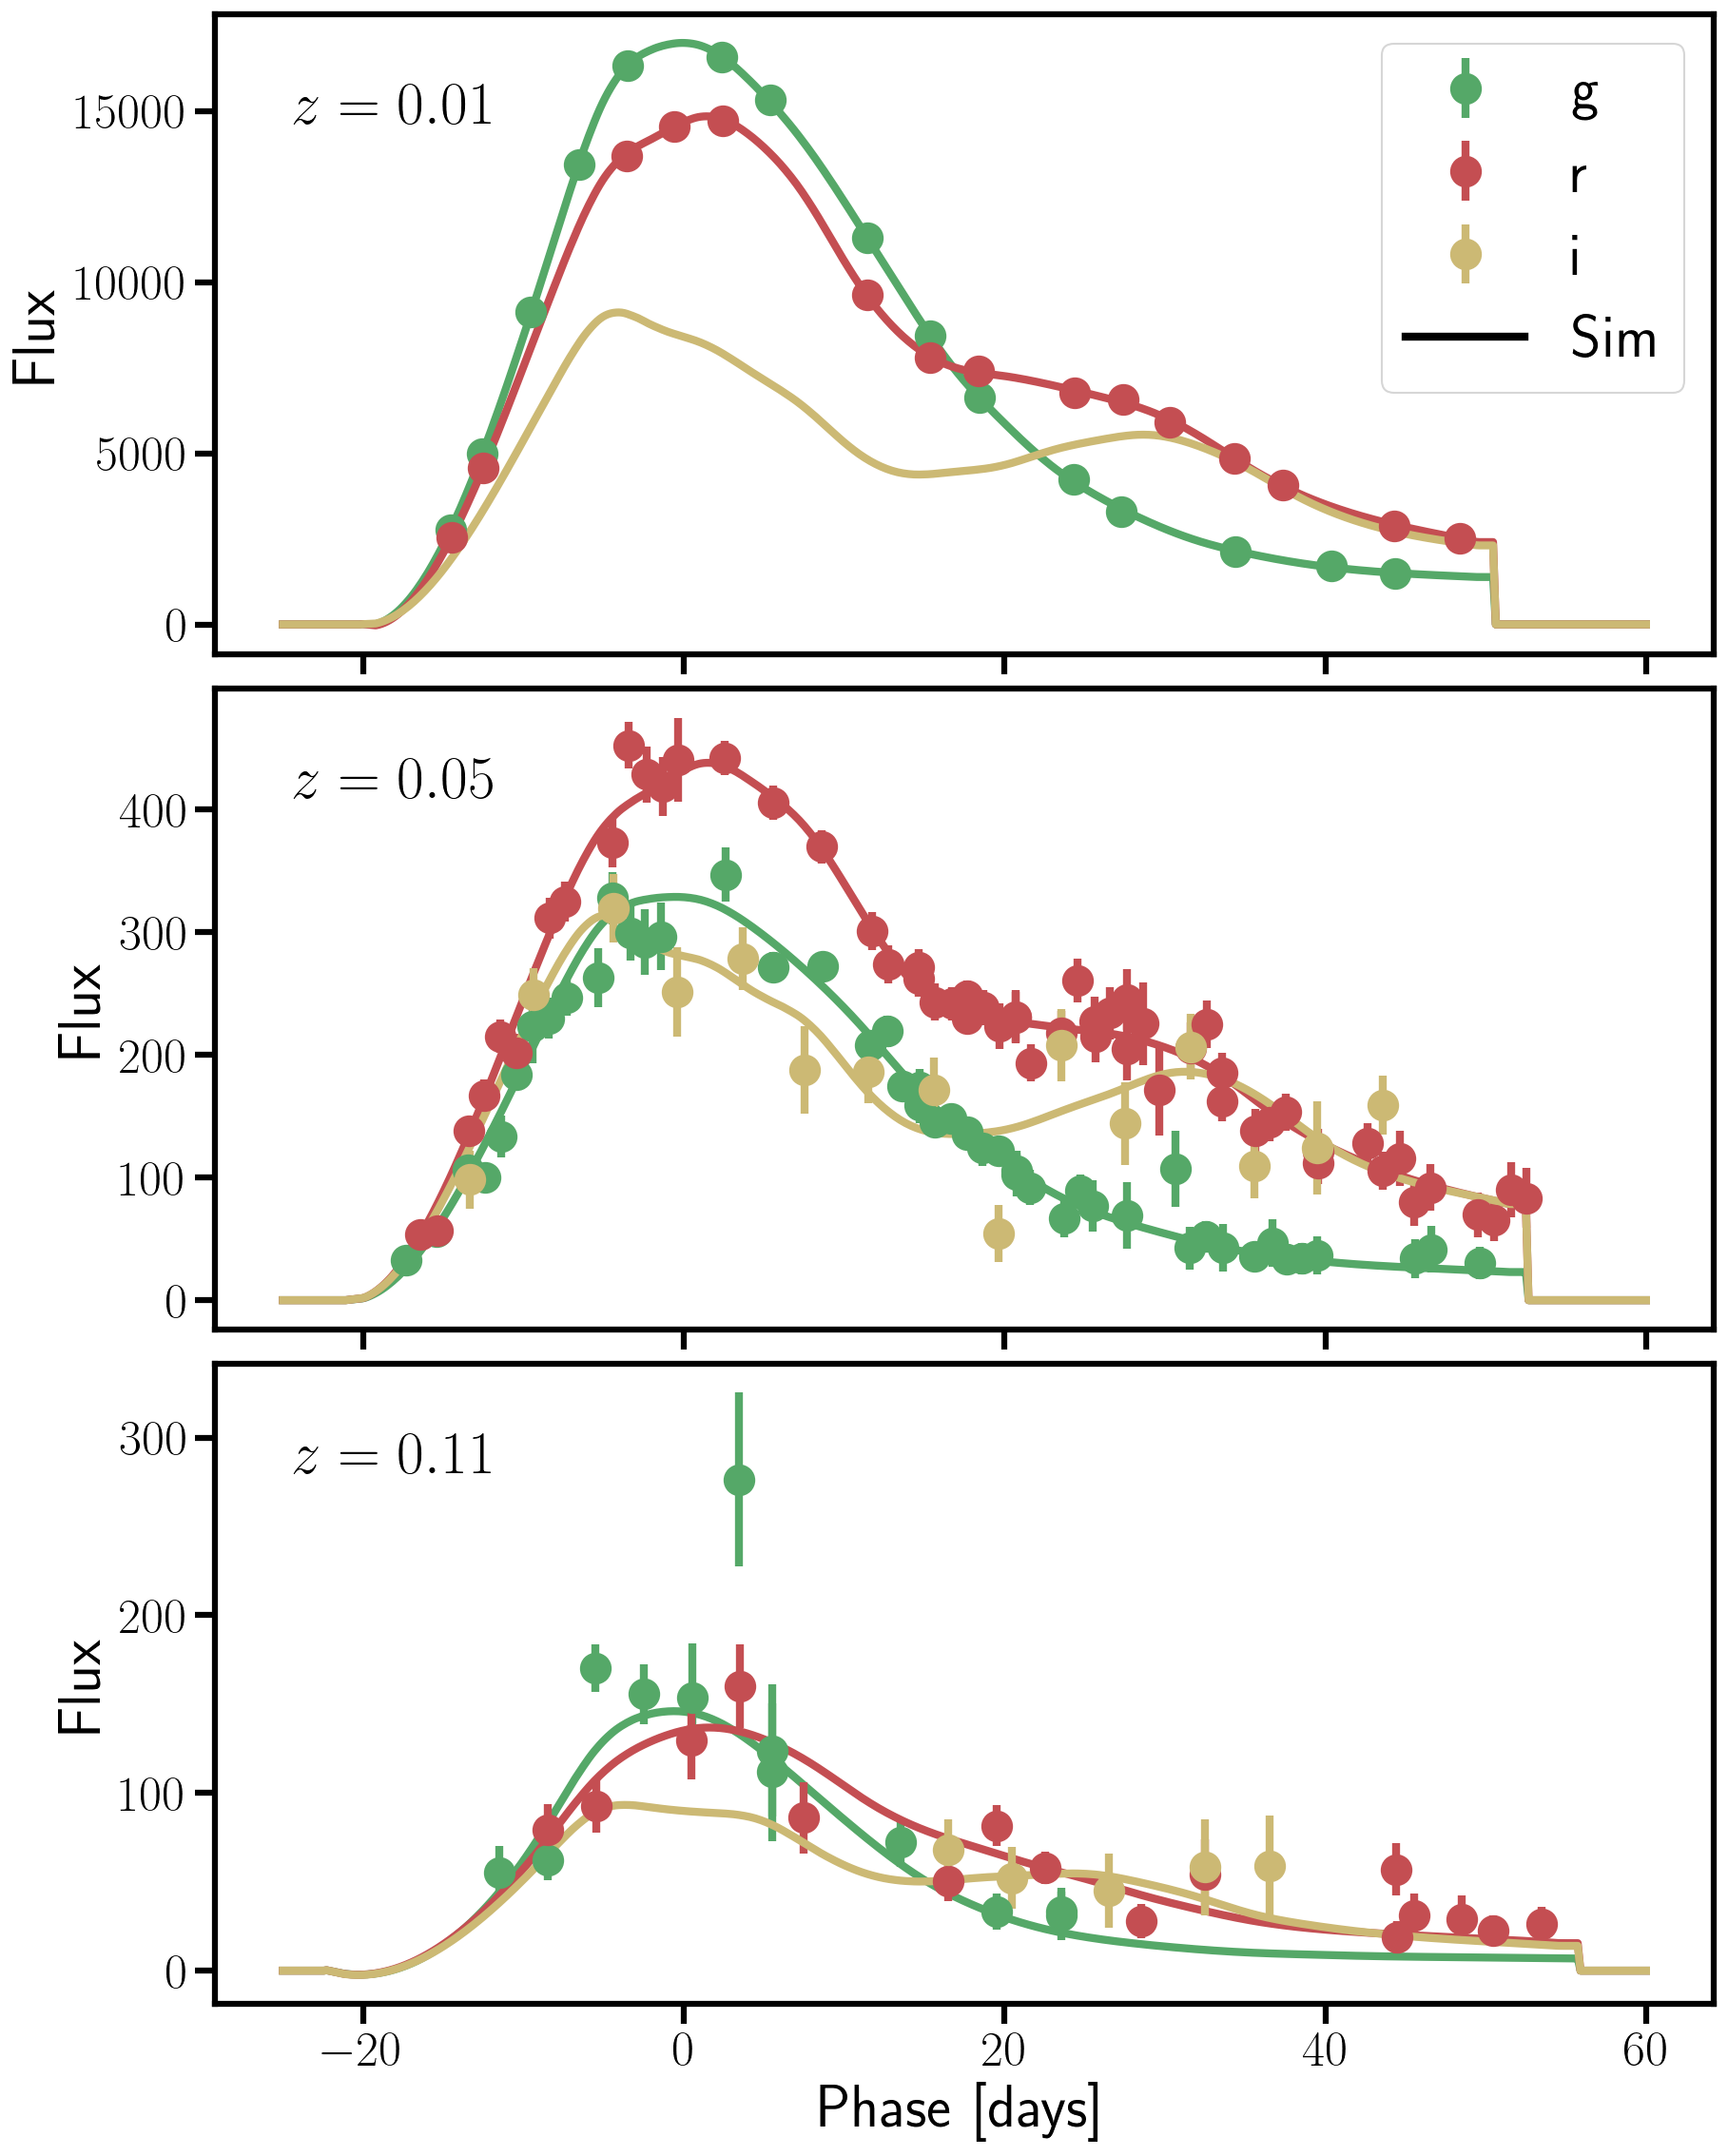
\includegraphics[width=0.6\textwidth]{fig/velocities/snsim_lightcurves.png}
    \caption{Three simulated type-Ia supernovae light-curves as observed by ZTF, ranging from low to mid and high redshift. 
    The solid line represents the input light-curve model while points with error bars are simulated observed fluxes 
    including instrumental noise. The flux is in arbitrary units. Figure extracted from Carreres et al. (in prep). }
    \label{fig:ztf_snsim_lightcurves}
\end{figure}

Figure~\ref{fig:ztf_snsim_hubble_diagram} displays the residuals of the Hubble diagram 
fitted on simulated samples of ZTF light-curves, relative to the true input Hubble diagram. 
The average of eight independent realisations is also displayed with error bars. 
A clear bias relative to the input model is seen at $z > 0.06$, 
due mainly to the selection for spectroscopic follow-up. 
If the simulations are realistic enough, this bias is an indication that ZTF SNIa samples 
are \emph{complete} up to $z \sim 0.06$, defining a so called \emph{volume limited} sample. 
Above this limit, we need to correctly 
account for biases if one is interested in constraining cosmology with the Hubble diagram. 
In this work, we studied the impact of this selection bias in the measurement of peculiar 
velocities and subsequently on the estimates of the growth-rate $f\sigma_8$.  

\begin{figure}[t]
    \centering
    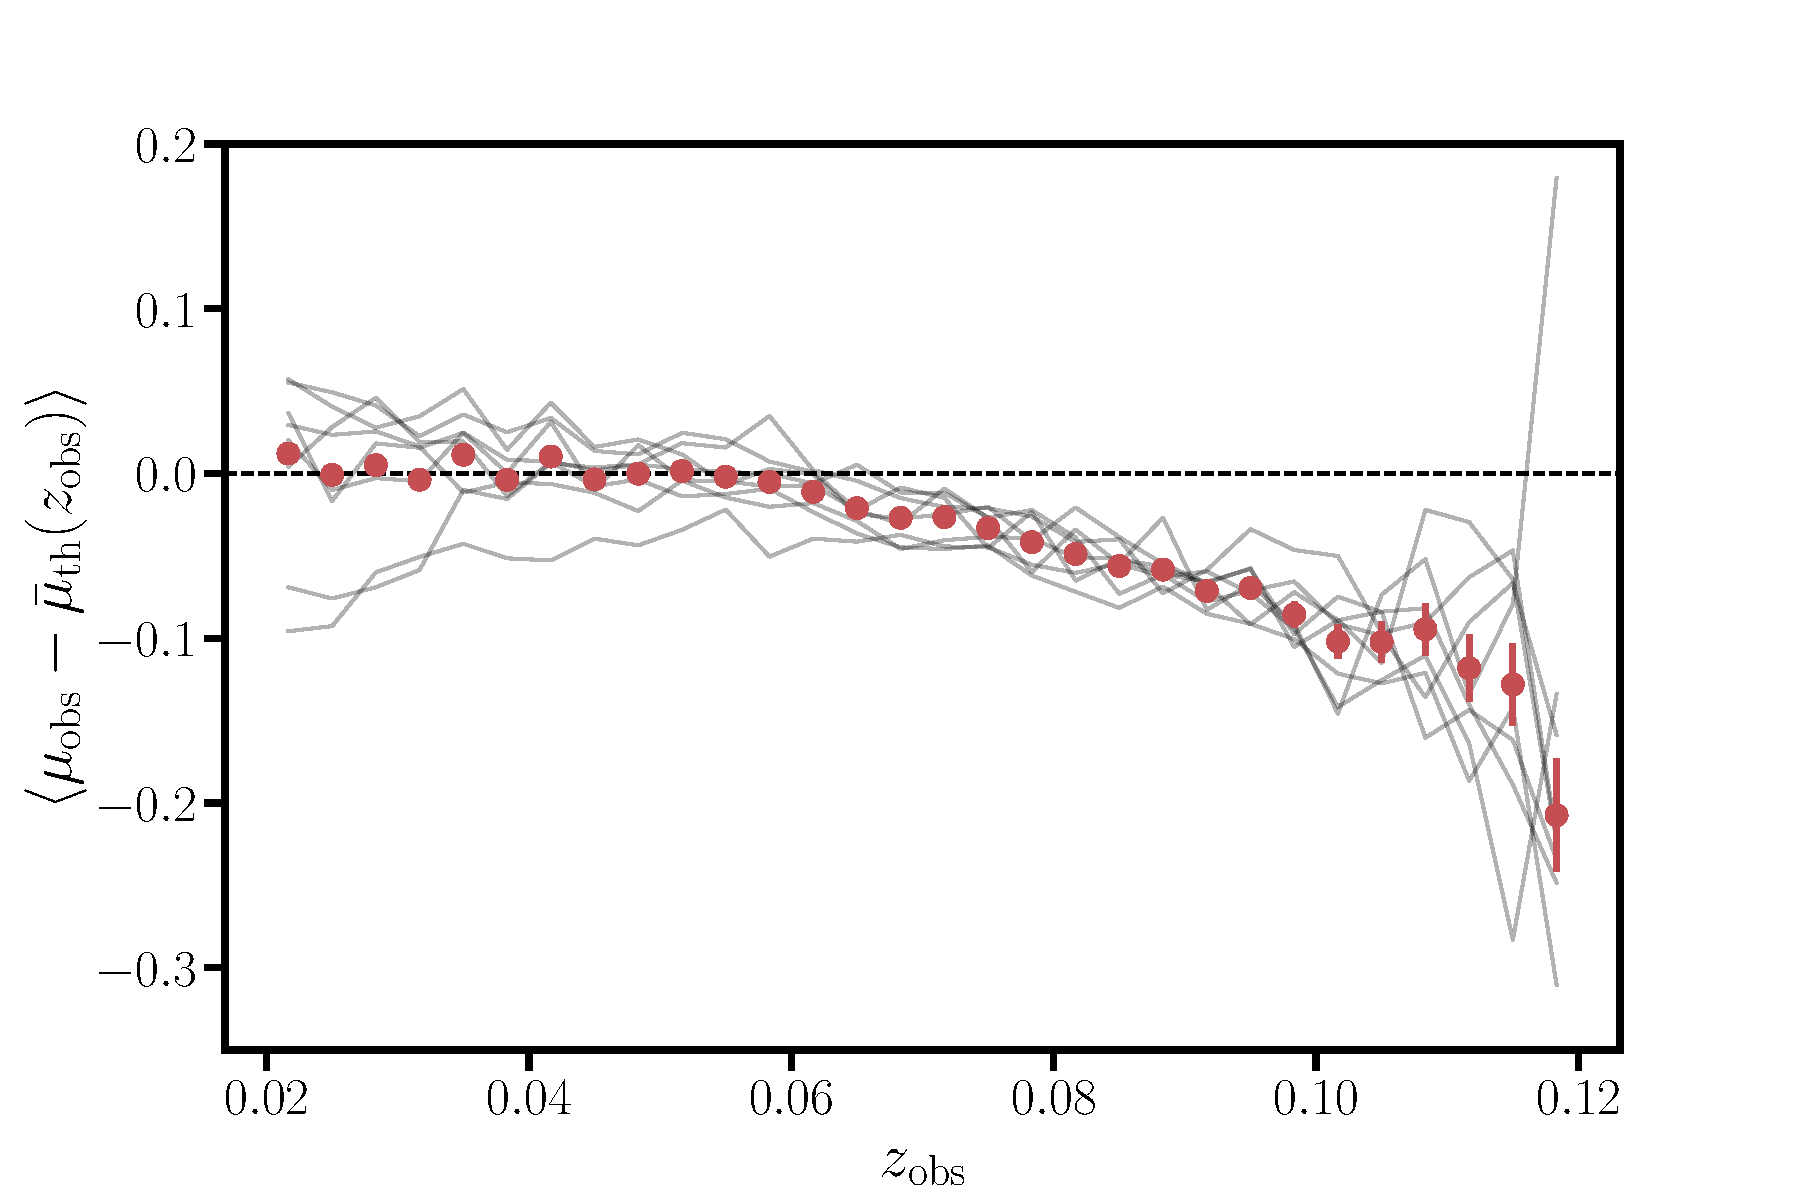
\includegraphics[width=0.6\textwidth]{fig/velocities/bastien_hd_residuals.pdf}
    \caption{Distance moduli inferred from simulated ZTF SNIa light-curves compared to the input cosmological model. 
    Grey lines show 8 different realisations while points with error bars are their average. 
    Selection effects cause a bias in distance moduli estimates at $z>0.06$. 
    Figure extracted from Carreres et al. (in prep).}
    \label{fig:ztf_snsim_hubble_diagram}
\end{figure}

For our measurement of $f\sigma_8$ using peculiar velocities, we are currently employing 
the maximum-likelihood method (section~\ref{velocities:methods:maximum_likelihood}). 
Instead of using a linear matter power spectrum as a model for the velocity divergence 
power spectrum, we are trying to use improved models including regularised perturbation 
theory (RegPT, \cite{taruyaDirectFastCalculation2012}) and empirical formulas derived
from n-body simulations (\cite{belAccurateFittingFunctions2019}). 
These models include some level of non-linearities which would allow us to use 
a larger range of scales when constraining growth. Also, linear theory is known to break 
at quite large scales $k\sim 0.1$, particularly at $z\sim0$. 

When building the model covariance matrix used in the likelihood (Eq.~\ref{eq:likelihood})
for $N_v$ measurements of peculiar velocities, the resulting matrix will have $N_v^2$ elements, 
which can become prohibitively large and slow to compute. We expect that ZTF will produce a set 
of about 5000 SNIa which is still feasible, but larger sets require a different solution. 
One of the solutions is to assign the velocities to a mesh, effectively reducing the number of 
measurements. This also has the advantage of smoothing out a fraction of the non-linear clustering. 
The mesh smoothing is taken into account in the model covariance matrix. 

There are three free parameters in the model covariance matrix: $f\sigma_8$ which is simply to overall 
amplitude of velocity-velocity correlations, $\sigma_v$ accounting for the remaining non-linear 
velocities, $\sigma_u$ accounting for the change in the signal due to redshift-space distortions. 
We use the \textsc{iMinuit} package\footnote{\url{https://iminuit.readthedocs.io/}} to find the maximum 
of the likelihood and to estimate uncertainties. We also explore the full posterior distribution 
using a Monte Carlo Markov Chain (MCMC). 

Figure~\ref{fig:ztf_snsim_posterior} shows one example of the posterior on the three fitter parameters. 
In order to avoid selection biases, we restrain our dataset to SNIa at $z<0.06$, 
which yields about 2000 objects for this case.
Contours show the 68 and 95\% confidence levels. Green contours are the result of analysing the 
peculiar velocities directly from the halo catalogue, without any source of noise. Red contours 
are the result when including all the effects of a realistic dataset and analysis. 
Both measurements are consistent with the expected value for $f\sigma_8$, even though uncertainties 
are quite large.

\begin{figure}[t]
    \centering
    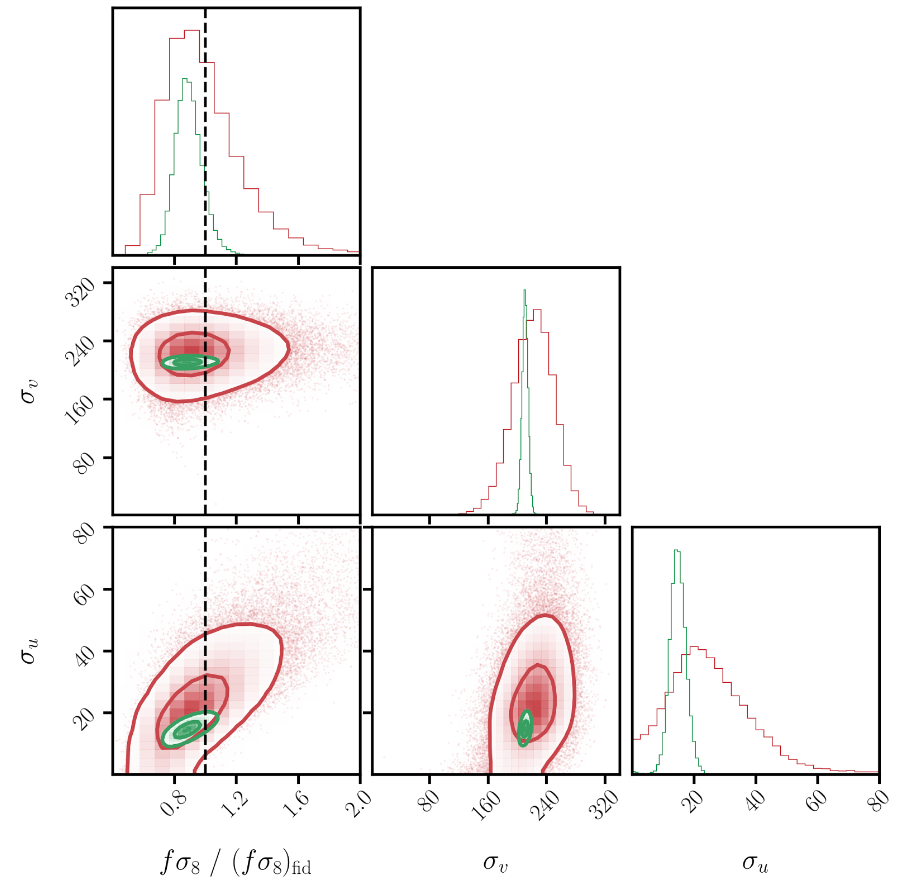
\includegraphics[width=0.6\textwidth]{fig/velocities/bastien_posterior_fs8.png}
    \caption{Example of posterior probability distribution for the growth-rate $f\sigma_8$ 
    and the dispersion parameters $\sigma_v$ and $\sigma_u$, obtained from an analysis 
    on a mock ZTF sample. Green contours are the result when halo radial peculiar velocities 
    are used directly without any source of noise. Red contours are the case of a full ZTF mock 
    SNIa catalogue, including light-curve simulation and fitting. The dashed vertical line represents
    the input value of the simulation.  
    Figure extracted from Carreres et al. (in prep).}
    \label{fig:ztf_snsim_posterior}
\end{figure}

Figure~\ref{fig:ztf_snsim_fs8_bias} shows how best-fit values of $f\sigma_8$ change when 
increasing the dataset up to $z_\text{max}$. We clearly see the impact of selection biases 
when considering SNIa beyond $z\sim 0.08$, based on the average of 8 mock realisations. 
This would indicate that an unbiased measurement of $f\sigma_8$ is possible with ZTF SNIa
if one restricts the analysis to the volume limited sample. 
Another interesting result is that the uncertainty in $f\sigma_8$ does not seem to 
decrease significantly when increasing $z_\text{max}$. This is simply a manifestation 
of the quick fall in the comoving density of SNIa beyond $z\sim0.08$, as seen in 
Figure~\ref{fig:nz_desi_ztf}. 
Also in the same redshift range, a large set of DESI galaxies will be available to 
perform a joint density-velocity analysis. 

\begin{figure}[t]
    \centering
    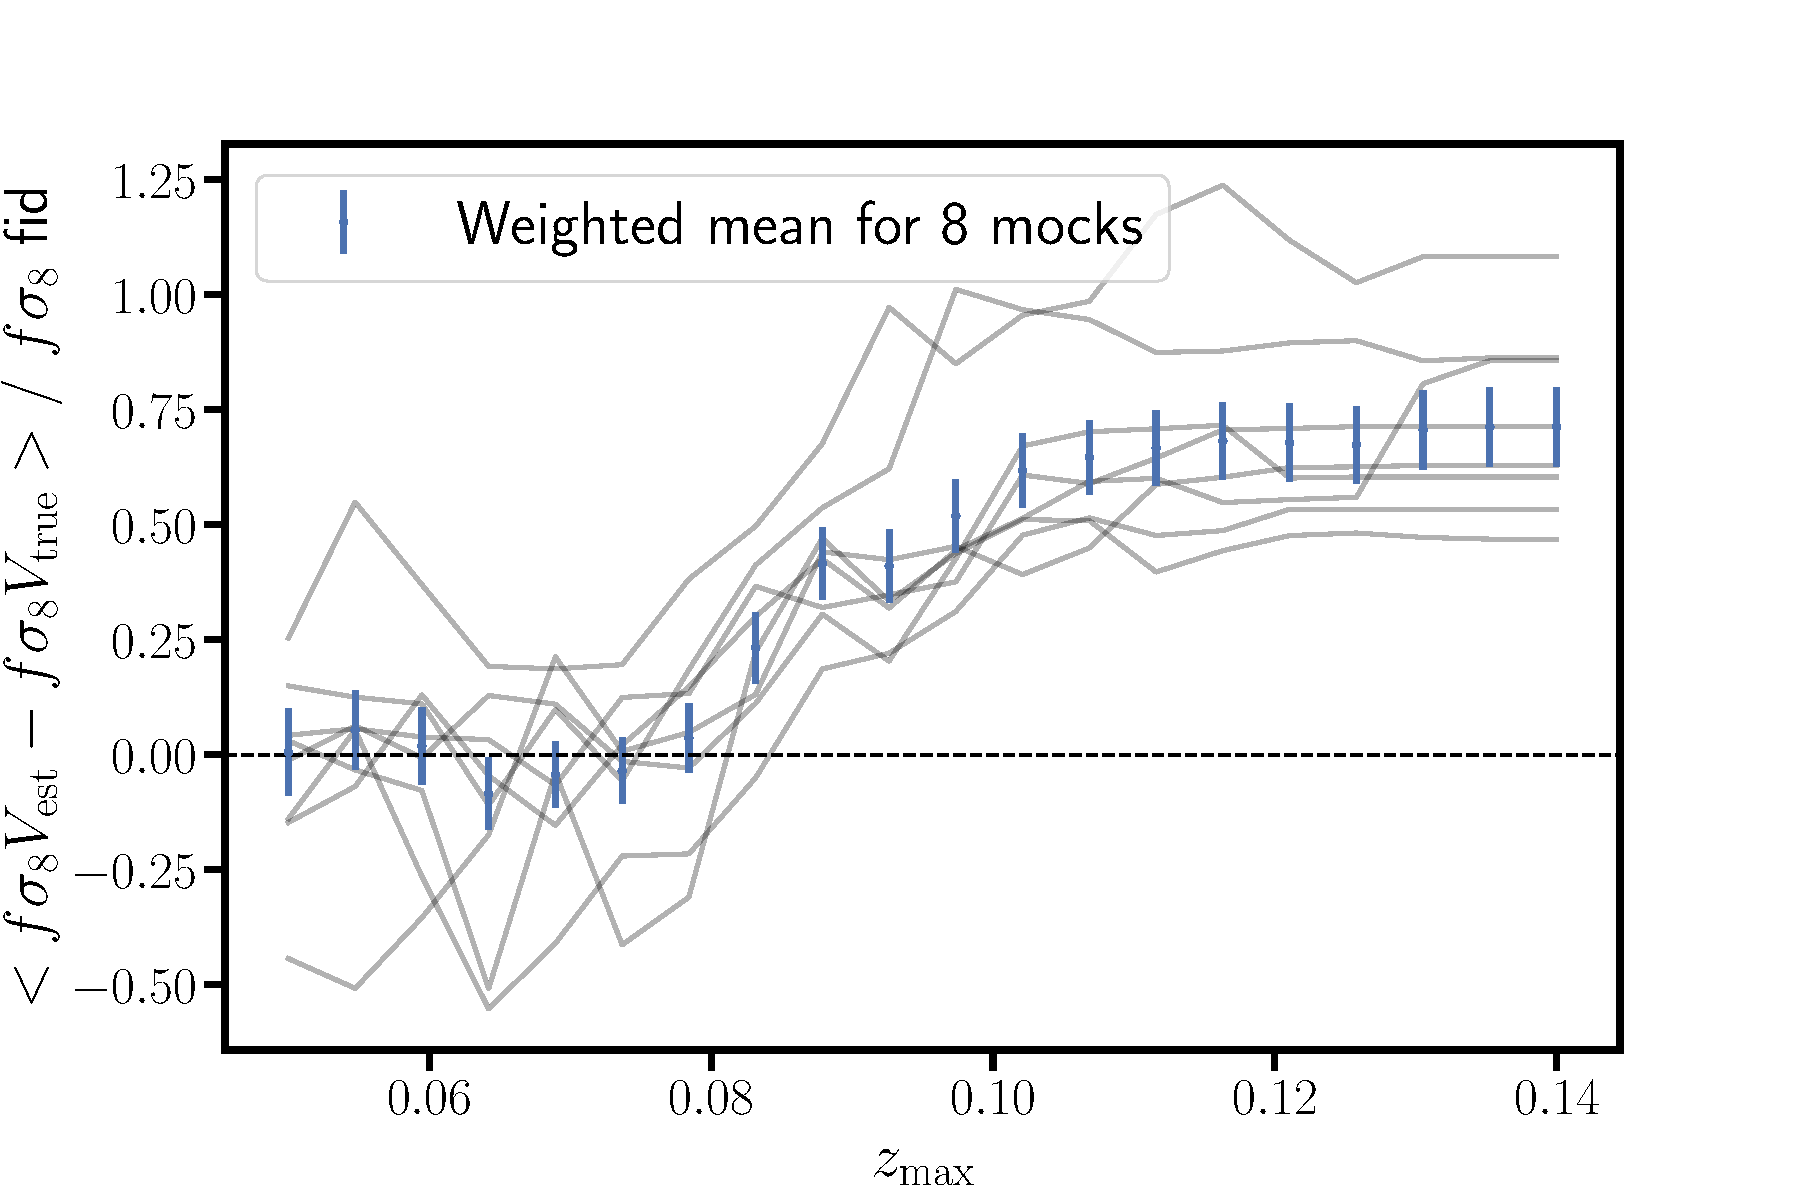
\includegraphics[width=0.6\textwidth]{fig/velocities/bastien_fs8_bias.pdf}
    \caption{Estimates of the growth-rate $f\sigma_8$ from mock ZTF SNIa data. 
    We compare the measurements between the estimated peculiar velocities to the 
    same measurements performed on the true velocities. 
    Each measurement considers SNIa up to maximum redshift $z_\text{max}$.
    The selection bias from Figure~\ref{fig:ztf_snsim_hubble_diagram} manifests itself
    on growth-rate estimates from $z_\text{max}>0.08$. 
    Figure extracted from Carreres et al. (in prep).}
    \label{fig:ztf_snsim_fs8_bias}
\end{figure}

